\documentclass[../../main.tex]{subfiles}
\begin{document}
\subsection{Software Lösungskonzepte}
Die Steuerungssoftware welche auf dem Hauptrechner ausgeführt wird soll in mehrere Teilprogramme aufgeteilt werden.
Einerseits können so die Teilprogramme unabhängig implementiert werden und andererseits einfacher getestet werden.
Um anschliessend zwischen den Teilprogrammen zu kommunizieren wird eine Middleware verwendet. Die Middleware kann auch genutzt werden
um die einzelnen Teilprogramme zu testen. Zusätzlich können verschiedene Programmiersprachen verwendet werden für die einzelnen Teilprogramme
was zusätzliche Flexibilität

\subsubsection{Architektur}
Im folgenden Diagramm wird die Architektur der Steuerungssoftware aufgezeigt
\begin{figure}[H] %Architektur mit Middleware
    \centering
    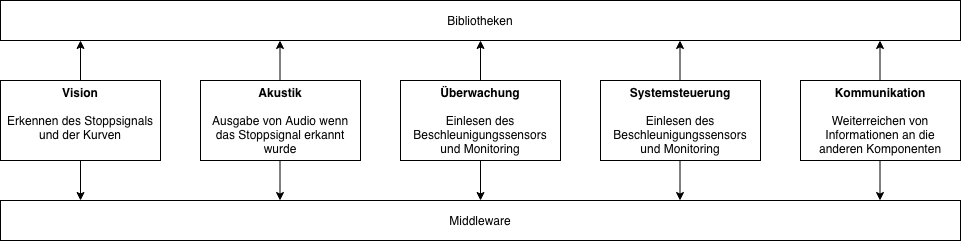
\includegraphics[width=1.0\textwidth]{drawings/ArchitekturDiagramm/SW_Architektur_Middleware.png}
    \caption {Software Architektur Middleware. Gezeichnet mit https://draw.io}
\end{figure}

\textbf{Legende:}
\begin{itemize}
    \item Die Pfeile visualisieren die Abhängigkeiten innerhalb der Architektur
\end{itemize}

\subsubsection{Technologie}
Während der Technologierecherche wurde eine Analyse gemacht um zu entscheiden welche Technologie eigesetzt werden soll. Bald wurde ZeroMQ
auserkoren da ZeroMQ schlank ist und ohne Performance Probleme auf kleinen Einplatinenrechner läuft. Ausserdem ist die Middleware bekannt
und hat eine hervorragende Dokumentation. Um die Daten welche über die Middleware geschickt werden mit verschiedenen Programmiersprachen zu
nutzen wird Protobuffers. Protobuffers ist ein Format zur Berschreibung von Daten. Dieses Format kann anschliessend verwendet werden um
Klassen bzw. Funktionen für fast jede Programmiersprache zu benutzen. Das heisst das die Daten einmalig definiert werden und anschliessend von
allen Teilprogrammen verwendet werden können.

\textbf{Beispiel Protobuf:}
\lstinputlisting{../src/raspi/pb/direction.proto}
Man sieht nun das eine 'Direction' Mitteilung definiert wird welche ein String Attribute hat welches direction heisst. Mit dieser Definition
nun mithilfe von einem 'protobuffer compiler' Code generiert werden welcher die definierte Message Serialisieren und Deserialisieren kann.

\textbf{Beispiel Generierung für Python:}
\begin{lstlisting}
    protoc -I=pb --python_out=pb pb/direction.proto
\end{lstlisting}
Mithilfe von diesem Beispiel wird die Protobuf Definition (direction.proto) zu Python Code generiert.

\textbf{Beispiel Generierter Python Code:}
\lstinputlisting[language=Python]{../src/raspi/pb/direction_pb2.py}
Das generierte Python File welches mithilfe des 'protobuffer compiler' erzeugt wurde.

\subsubsection{Proof-of-Concept}
Um zu testen ob eine Kommunikation zwischen zwei Prozessen mithilfe der Middleware möglich ist wurde eine kleine Testsoftware entwickelt.
Dabei wurde das 'direction.proto' File verwendet um vom einten Prozess eine Richtung (Direction) zu einem anderen Prozess zu senden.

Der Sender der Richtung wurde im folgenden File implementiert: src/raspi/vision/linedetection/fakelinedetector.py
Der Empfänger der Richtung wurde im folgenden File implementiert: src/raspi/webapp/middlewareadapter.py
wobei der Empfänger von vom Webapp Server gestartet wird: src/raspi/webapp/server.py

\subsubsection{Performance}
Die Performance wurde nicht selbst gemessen und verifiziert. Jedoch wurden bei unseren Tests keine Limitationen gefunden und deshalb gehen wir davon aus
das die Performance für unseren Anwendungsfall ausreicht. Ausserdem werden nur wichtige Events zwischen den Prozessen ausgetauscht und somit ist die Datenrate
eher zweitrangig. Die Latenz ist jedoch sehr zentral um einen möglichst agilen Regelkreis zu implementieren. Hier bewegt sich ZeroMQ zwischen 450us - 700us.

\textbf{Performance Tests:}
\begin{itemize}
    \item http://zeromq.org/area:results
    \item http://nikolaveber.blogspot.com/2011/04/if-you-are-planning-large-or-not-even.html
\end{itemize}

\end{document}